\documentclass[../../main.tex]{subfiles}
\begin{document}

\chapter{Preliminaries}\label{chap:preliminaries}

\section{Notation and Conventions}
\label{sec:notation-conventions}

We work over the field $\mathbb{K}\in\{\mathbb{R},\mathbb{C}\}$. Statements that require $\mathbb{C}$ are indicated explicitly.

Vectors are column vectors unless otherwise stated. For $\mathbf{x},\mathbf{y}\in\mathbb{K}^n$ the inner product is
\[
    \langle \mathbf{x},\mathbf{y}\rangle := \mathbf{y}^H \mathbf{x},
\]
which is conjugate-linear in the first argument and linear in the second.

We define the associated Euclidean 2-norm as our standard norm $\|\cdot\| = \|\cdot\|_2$, unless otherwise specified:
\[
    \|\mathbf{x}\|_2=\sqrt{\langle\mathbf{x},\mathbf{x}\rangle}.
\]

For matrices $A\in\mathbb{K}^{m\times n}$ we use
\begin{itemize}
    \item $A^H$ for the conjugate transpose, and $A^T$ for the (real) transpose,
    \item $\overline{A}$ or $\overline{z}$ for elementwise complex conjugation,
    \item $I_n$ for the $n\times n$ identity and $0$ for a suitably sized zero matrix/vector,
    \item $A_{i,j}$ (or $[A]_{ij}$) for the $(i,j)$ entry and $A_{p:q,r:s}$ for the submatrix with row indices $p,\dots,q$ and column indices $r,\dots,s$,
    \item $\operatorname{diag}(d_1,\dots,d_n)$ for a diagonal matrix with the given diagonal entries.
\end{itemize}

Matrix norms and spectral quantities:
\[
    \|A\|_2 := \max_{\|\mathbf{x}\|_2=1}\|A\mathbf{x}\|_2 \qquad\text{(spectral/operator 2-norm)},
\]
\[
    \|A\|_F := \sqrt{\sum_{i,j}|a_{ij}|^2}\qquad\text{(Frobenius norm)},
\]
\[
    \rho(A) := \max_i |\lambda_i(A)|\qquad\text{(spectral radius)}.
\]

Other common notation:
\begin{itemize}
    \item $e_i$ denotes the $i$th standard basis vector in $\mathbb{K}^n$ and $\mathbf{e}=(1,\dots,1)^\top$,
    \item $\operatorname{tr}(A)$ denotes the trace, $\det(A)$ the determinant, and $\operatorname{rank}(A)$ the rank,
    \item $\Re(z)$ and $\Im(z)$ denote the real and imaginary parts of a complex number $z$,
    \item for sequences/functions we use standard asymptotic notation ($O(\cdot), o(\cdot)$) when needed.
\end{itemize}

These conventions are used throughout the text; any deviation will be stated where it occurs.

\section{Matrices}
\label{sec:matrices}

\subsection{Eigenvalues and Eigenvectors}
\label{subsec:eigs}
Let $A\in\mathbb{C}^{n\times n}$. A scalar $\lambda\in\mathbb{C}$ and nonzero vector $\mathbf{v}\in\mathbb{C}^n$ satisfy
\[
    A\mathbf{v}=\lambda\mathbf{v}\qquad\text{(right eigenpair)}.
\]
Left eigenvectors $\mathbf{w}$ satisfy $\mathbf{w}^H A = \lambda \, \mathbf{w}^H$, equivalently $A^H\mathbf{w}=\overline{\lambda}\,\mathbf{w}$. If $A$ is Hermitian ($A^H=A$), all eigenvalues are real; if $A$ is singular, $0$ is an eigenvalue.

\subsection{Image (Range) and Kernel (Nullspace)}
\label{subsec:image-kernel}

\begin{definition}{Image / Range}{image}
    The \emph{image} (or \emph{range}) of $A\in\mathbb{R}^{m\times n}$ is
    \[
        \operatorname{Im}(A)=\{A\mathbf{x}:\mathbf{x}\in\mathbb{R}^n\} =\operatorname{span}\{\mathbf{a}_1,\dots,\mathbf{a}_n\},
    \]
    where $\mathbf{a}_j$ are the columns of $A$. The \emph{rank} of $A$ is
    \[
        \operatorname{rank}(A)=\dim(\operatorname{Im}(A)).
    \]
\end{definition}

\begin{definition}{Kernel / Null space}{nullspace}
    The \emph{kernel} (or \emph{null space}) of $A\in\mathbb{R}^{m\times n}$ is
    \[
        \ker(A)=\{\mathbf{x}\in\mathbb{R}^n: A\mathbf{x}=\mathbf{0}\}.
    \]
    Its dimension is the \emph{nullity} of $A$:
    \[
        \operatorname{nullity}(A)=\dim(\ker(A)).
    \]
\end{definition}

\begin{theorem}{Rank-Nullity Theorem}{rank-nullity-theorem}
    For any matrix $A\in\mathbb{R}^{m\times n}$,
    \[
        \operatorname{rank}(A)+\operatorname{nullity}(A)=n.
    \]
\end{theorem}

\begin{proof}[Proof sketch]
    Consider the linear map $x\mapsto Ax$. Choose a basis of $\ker(A)$ and extend it to a basis of $\mathbb{R}^n$. The remaining basis vectors map to a basis of $\operatorname{Im}(A)$, giving the stated equality.
\end{proof}

Immediate consequences of the rank-nullity theorem are:
\begin{itemize}
    \item $A$ has full column rank iff $\ker(A)=\{0\}$.
    \item If $m<n$ then $\ker(A)\neq\{0\}$ for rank-deficient $A$ (pigeonhole).
    \item Solutions of $A\mathbf{x}=\mathbf{b}$ exist iff $\mathbf{b}\in\operatorname{Im}(A)$; when solutions exist they form an affine space $\mathbf{x}_0+\ker(A)$.
\end{itemize}

\subsection{Normal Matrices}
\label{subsec:normal-matrices}

A matrix $A \in \mathbb{C}^{n \times n}$ is \emph{normal} if
\[
    AA^H = A^H A,
\]
For real matrices, this becomes $AA^T = A^TA$.

Normal matrices are special because they \emph{commute} with their conjugate transpose; meaning $A A^H = A^H A$. This property guarantees that the matrix has a complete set of orthogonal eigenvectors.

\begin{remark}{Intuition for Normal Matrices}{intuition-normal-matrices}
    Think of Normal Matrices like this: most matrices will stretch, rotate, AND skew vectors in complicated ways. But normal matrices are \emph{well-behaved}, they only stretch or shrink along specific perpendicular directions, without mixing them up. This makes them much easier to understand and work with.
\end{remark}

\begin{theorem}{Spectral Theorem for Normal Matrices}{spectral-normal}
    A matrix $A \in \mathbb{C}^{n \times n}$ is normal if and only if it admits a unitary diagonalization:
    \[
        A = U D U^H,
    \]
    where $U \in \mathbb{C}^{n \times n}$ is unitary ($U^H U = I$) and $D = \text{diag}(\lambda_1, \ldots, \lambda_n)$ contains the eigenvalues.
\end{theorem}

This characterization shows that normal matrices are precisely those with a complete orthonormal basis of eigenvectors. The geometric intuition is that normal matrices preserve orthogonality when acting on their eigenspaces.

\paragraph{Important subclasses of normal matrices:}
\begin{description}
    \item[Hermitian matrices:] $A = A^H$, which implies all eigenvalues are real: $\lambda_i \in \mathbb{R}$.
    \item[Skew-Hermitian matrices:] $A = -A^H$, which implies all eigenvalues are purely imaginary: $\lambda_i \in i\mathbb{R}$.
    \item[Unitary matrices:] $A^H A = I$, which implies all eigenvalues have unit modulus: $|\lambda_i| = 1$.
\end{description}

\subsection{Hermitian Matrices}

\begin{definition}{Hermitian (Self-adjoint)}{hermitian}
    A matrix $A \in \mathbb{C}^{n \times n}$ is \emph{Hermitian}(or \emph{self-adjoint}) if
    \[
        A = A^H,
    \]
    that is, $A$ equals its conjugate transpose. Over the reals, this condition reduces to symmetry: $A = A^\top$.
\end{definition}

\begin{remark}{Intuition}{intuition-hermitian}
    Hermitian matrices are the complex analogue of real symmetric matrices.
    They have a built-in geometric symmetry: being equal to their own conjugate transpose makes them “balanced” across the main diagonal.
    This structure guarantees real eigenvalues and an orthonormal eigenbasis, which makes Hermitian matrices highly predictable and stable compared to general matrices.
\end{remark}

\begin{theorem}{Spectral Theorem for Hermitian Matrices}{spectral-hermitian}
    If $A \in \mathbb{C}^{n \times n}$ is Hermitian, then:
    \begin{enumerate}
        \item All eigenvalues are real: $\lambda_i \in \mathbb{R}$.
        \item There exists an orthonormal basis of eigenvectors.
        \item $A$ admits a unitary diagonalization:
              \[
                  A = U D U^H,
              \]
              where $U$ is unitary and $D$ is a real diagonal matrix of eigenvalues.
    \end{enumerate}
\end{theorem}

\begin{proof}[Proof sketch: eigenvalues are real]
    Let $\lambda$ be an eigenvalue of $A$ with eigenvector $\mathbf{v} \neq 0$. Then
    \[
        \lambda \|\mathbf{v}\|^2
        = \lambda \mathbf{v}^H \mathbf{v}
        = \mathbf{v}^H A \mathbf{v}
        = \mathbf{v}^H A^H \mathbf{v}
        = (A\mathbf{v})^H \mathbf{v}
        = (\lambda \mathbf{v})^H \mathbf{v}
        = \overline{\lambda}\, \|\mathbf{v}\|^2.
    \]
    Since $\|\mathbf{v}\|^2 > 0$, we conclude $\lambda = \overline{\lambda}$, hence $\lambda \in \mathbb{R}$.
\end{proof}

\paragraph{Variational characterization.}
For Hermitian $A$, the eigenvalues sorted nonincreasingly satisfy the \emph{min-max principle}:
\[
    \lambda_k(A)=\min_{\dim S=k}\ \max_{\substack{\mathbf{x}\in S\\ \|\mathbf{x}\|=1}} \mathbf{x}^H A \mathbf{x}.
\]
The Rayleigh quotient $R_A(\mathbf{x})=\dfrac{\mathbf{x}^H A \mathbf{x}}{\mathbf{x}^H \mathbf{x}}$ obeys $\min R_A=\lambda_n$, $\max R_A=\lambda_1$.

\paragraph{Computational advantages.}
Hermitian structure halves storage, enables real arithmetic when $A\in\mathbb{R}^{n\times n}$, and admits stable, cost-effective eigenvalue algorithms (e.g., tridiagonal reduction + QR). Perturbation theory is particularly benign: eigenvalues satisfy Weyl's theorem; eigenvectors obey Davis-Kahan bounds when eigenvalue gaps are present.

\begin{example}{Quadratic Forms}{quadratic-forms}
    For Hermitian $A$ and vector $\mathbf{x}$, the quadratic form $\mathbf{x}^H A \mathbf{x}$ is always real. Using the spectral decomposition:
    \[
        \mathbf{x}^H A \mathbf{x} = \mathbf{x}^H U D U^H \mathbf{x} = \sum_{i=1}^n \lambda_i |u_i^H \mathbf{x}|^2
    \]
    This shows how the eigenvalues directly control the behavior of the quadratic form.
\end{example}

The special structure of normal and Hermitian matrices makes them the foundation for many numerical algorithms, from eigenvalue computation to optimization methods that rely on their predictable spectral behavior.

\subsection{Nonnegative Matrices}
Nonnegative matrices are widely used in applications involving positive quantities, such as probability distributions, population dynamics, economic models, and network analysis. Their spectral properties are described by the Perron-Frobenius theory, which governs their eigenvalue structure.

\begin{definition}{Nonnegative Matrix}{nonnegative-matrix}
    A matrix $A \in \mathbb{R}^{n \times n}$ is \emph{nonnegative} if $a_{ij} \geq 0$ for all $i, j$. We write $A \geq 0$.

    A matrix is \emph{positive} if $a_{ij} > 0$ for all $i, j$, denoted $A > 0$.
\end{definition}

\begin{theorem}{Perron-Frobenius Theorem}{perron-frobenius}
    Let $A \geq 0$ be a nonnegative matrix. Then:
    \begin{enumerate}
        \item The spectral radius $\rho(A) = \max_i |\lambda_i|$ is an eigenvalue of $A$.
        \item There exists a nonnegative eigenvector $\mathbf{x} \geq 0$ such that $A\mathbf{x} = \rho(A)\mathbf{x}$.
        \item If $A$ is irreducible, then $\rho(A)$ is a simple eigenvalue, and there exists a positive eigenvector $\mathbf{x} > 0$ such that $A\mathbf{x} = \rho(A)\mathbf{x}$.
        \item If $A$ is irreducible and aperiodic, then $\rho(A)$ is the unique eigenvalue of maximum modulus, i.e., $|\lambda| < \rho(A)$ for all other eigenvalues $\lambda$.
    \end{enumerate}
\end{theorem}

The Perron-Frobenius theorem guarantees that nonnegative matrices have a dominant eigenvalue $\rho(A)$, which is real and positive.
This eigenvalue corresponds to a nonnegative eigenvector, and in the case of irreducibility, a strictly positive eigenvector.

The dominant eigenvalue $\rho(A)$ often represents the long-term growth rate or stability of the system described by $A$.

\subsection{Kantorovich Inequality}\label{subsec:kantorovich-inequality}

Kantorovich inequality provides bounds on the relationship between different norms induced by a symmetric positive definite matrix.
\begin{theorem}{Kantorovich Inequality}{kantorovich}
    Let $B \in \mathbb{R}^{n \times n}$ be SPD with eigenvalues $0 < \lambda_1 \leq \cdots \leq \lambda_n.$
    Then for all $\mathbf{x} \in \mathbb{R}^n$,
    \[
        \frac{\|\mathbf{x}\|_B^2 \,\|\mathbf{x}\|_{B^{-1}}^2}{\|\mathbf{x}\|_2^4}
        \leq \frac{1}{4}\cdot\frac{(\lambda_1 + \lambda_n)^2}{\lambda_1 \lambda_n}.
    \]
\end{theorem}
\begin{proof}
    Since $B$ is SPD, diagonalize $B = Q^{\top}\Lambda Q$ with $\Lambda = \operatorname{diag}(\lambda_1, \ldots, \lambda_n)$ and $Q$ orthogonal.
    For $y = Q\mathbf{x}$ with $\|\mathbf{x}\|_2 = \|y\|_2 = 1$:
    \begin{align*}
        B^{-1}                    & = Q^{\top} \Lambda^{-1} Q,                                                 \\
        \|\mathbf{x}\|_B^2        & = \mathbf{x}^{\top} B \mathbf{x} = \sum_{i=1}^n \lambda_i y_i^2,           \\
        \|\mathbf{x}\|_{B^{-1}}^2 & = \mathbf{x}^{\top} B^{-1} \mathbf{x} = \sum_{i=1}^n \lambda_i^{-1} y_i^2.
    \end{align*}

    Thus $\big(\bar\lambda, \bar\lambda^{-1}\big)$ with
    \[
        \bar\lambda = \sum_{i=1}^n \lambda_i y_i^2,
        \qquad
        \bar\lambda^{-1} = \sum_{i=1}^n \lambda_i^{-1} y_i^2,
    \]
    is a convex combination of points $(\lambda_i, 1/\lambda_i)$.

    The curve $1/\lambda$ is convex on $(0,\infty)$, hence
    \[
        \big(\bar\lambda, \bar\lambda^{-1}\big)
    \]
    lies below the chord
    \[
        \ell(\lambda) = \frac{1}{\lambda_1} + \frac{1}{\lambda_n} - \frac{\lambda}{\lambda_1 \lambda_n},
        \qquad \ell(\lambda_1) = \tfrac{1}{\lambda_1}, \;\; \ell(\lambda_n) = \tfrac{1}{\lambda_n}.
    \]
    Therefore
    \[
        \bar\lambda^{-1} \leq \ell(\bar\lambda).
    \]
    The maximum of $q(\bar\lambda) = \bar\lambda\,\ell(\bar\lambda)$ occurs at $\bar\lambda = \tfrac{1}{2}(\lambda_1 + \lambda_n)$, yielding
    \[
        \bar\lambda \,\bar\lambda^{-1} \leq \max_{\bar\lambda \in [\lambda_1, \lambda_n]} q(\bar\lambda) = \frac{(\lambda_1 + \lambda_n)^2}{4 \lambda_1 \lambda_n}
    \]\qed
\end{proof}

\begin{figure}[ht]
    \centering
    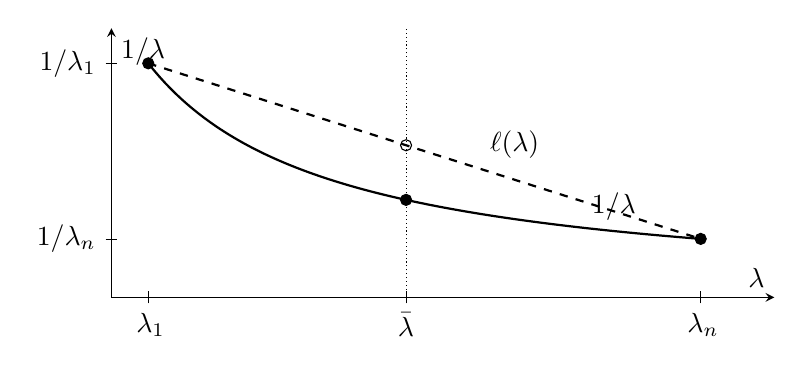
\begin{tikzpicture}
    \begin{axis}[
            width=10cm, height=6.2cm,
            axis lines=middle,
            xmin=0.8, xmax=4.4,
            ymin=0,   ymax=1.15,
            xlabel={$\lambda$}, ylabel={$1/\lambda$},
            xtick={1,2.4,4},
            xticklabels={$\,\lambda_1$, $\bar\lambda$, $\,\lambda_n$},
            ytick={1,0.25},
            yticklabels={$1/\lambda_1$, $1/\lambda_n$},
            tick style={black},
            width=10cm, height=5cm
        ]
        % curve y = 1/x
        \addplot[thick, samples=100, domain=1:4] {1/x} node[pos=0.85, above] {$1/\lambda$};

        % chord between (\lambda_1,1/\lambda_1) and (\lambda_n,1/\lambda_n)
        \addplot[thick, dashed, domain=1:4, samples=2]
        {(1/1) + ((1/4)-(1/1))*((x-1)/(4-1))}
        node[pos=0.6, above right] {$\ell(\lambda)$};

        % endpoints
        \addplot[only marks, mark=*] coordinates {(1,1) (4,0.25)};

        % bar-lambda marks
        \addplot[densely dotted] coordinates {(2.4,0) (2.4,1.2)};
        \addplot[only marks, mark=*] coordinates {(2.4,{1/2.4})}; % point on curve
        \addplot[only marks, mark=o] coordinates {(2.4,{ (1/1) + ((1/4)-(1/1))*((2.4-1)/(4-1)) })}; % point on chord

        % label
        \node[below] at (axis cs:2.4,0) {$\bar\lambda$};
    \end{axis}
\end{tikzpicture}
    \caption{Kantorovich inequality visualized via the convexity of $1/\lambda$ and its chord between $\lambda_1$ and $\lambda_n$.}
\end{figure}

\subsection{M-matrices}
M-matrices are matrices with nonpositive off-diagonal entries and a nonnegative inverse.
They ensure stability and monotonicity, making them useful in numerical analysis, optimization, and modeling problems with positivity constraints.

\begin{definition}{M-matrix}{m-matrix}
    A matrix $A \in \mathbb{R}^{n \times n}$ is an \emph{M-matrix} if:
    \begin{enumerate}
        \item $a_{ij} \leq 0$ for all $i \neq j$ (nonpositive off-diagonal entries)
        \item $A$ is nonsingular
        \item $A^{-1} \geq 0$ (nonnegative inverse)
    \end{enumerate}
\end{definition}

\begin{corollary}{M-matrix characterization}{m-matrix-characterization}
    An M-matrix can be written as $A = sI - B$ where $s > \rho(B)$ and $B \geq 0$.
\end{corollary}

\subsubsection{Properties of M-matrices}
Let $A$ be an M-matrix. Then:
\begin{enumerate}
    \item All eigenvalues have positive real parts: $\operatorname{Re}(\lambda_i) > 0$ for all $i$.
    \item All principal minors are positive: $\det(A_{ij}) > 0$ for all principal submatrices $A_{ij}$.
    \item $A$ is positive stable: solutions to $\mathbf{x}' = -A\mathbf{x}$ decay exponentially.
    \item The linear system $A\mathbf{x} = \mathbf{b}$ with $\mathbf{b} \geq 0$ has solution $\mathbf{x} \geq 0$.
\end{enumerate}

Their positive inverse property makes them particularly well-suited for iterative solution methods, as they preserve nonnegativity and ensure convergence.

\begin{example}{Discrete Laplacian as M-matrix}{discrete-laplacian}
    Consider the discrete 1D Laplacian on $n$ interior points with Dirichlet boundary conditions:
    \[
        A = \frac{1}{h^2} \begin{bmatrix}
            2  & -1 &        &        &        \\
            -1 & 2  & -1     &        &        \\
               & -1 & 2      & -1     &        \\
               &    & \ddots & \ddots & \ddots \\
               &    &        & -1     & 2
        \end{bmatrix}
    \]

    This matrix satisfies the M-matrix conditions: the diagonal entries are positive, off-diagonal entries are nonpositive, and the matrix is positive definite (hence $A^{-1} > 0$). This structure ensures that the discrete maximum principle holds for the corresponding difference equations.
\end{example}


\subsection{Unitary Matrices}

A matrix $Q \in \mathbb{C}^{n \times n}$ is \emph{unitary} if $Q^H Q = I_n$, where $I_n$ is the $n \times n$ identity matrix. The columns of $Q$ form an orthonormal set, meaning they are mutually orthogonal and each has unit norm.

Let $Q = [q_1, q_2, \ldots, q_n]$. Then the orthonormality condition is:
\begin{equation}
    (q_i, q_j) = \delta_{ij} = \begin{cases}
        1 & \text{if } i = j    \\
        0 & \text{if } i \neq j
    \end{cases}
\end{equation}

\subsubsection{Examples of Unitary Matrices}

\begin{enumerate}
    \item \textbf{Identity matrix}: $I_n$ is trivially unitary.

    \item \textbf{2D rotation matrices} (real orthogonal):
          \begin{equation}
              R(\theta) = \begin{bmatrix}
                  \cos(\theta) & -\sin(\theta) \\
                  \sin(\theta) & \cos(\theta)
              \end{bmatrix}
          \end{equation}
          Verification: $R(\theta)^T R(\theta) = I_2$ since $\cos^2(\theta) + \sin^2(\theta) = 1$.

    \item \textbf{Givens rotation}: $G(i,j,\theta)$ rotates components $i$ and $j$ by angle $\theta$:
          \begin{equation}
              G(i,j,\theta) = \begin{bmatrix}
                  I_{i-1} &   &    &         \\
                          & c & -s &         \\
                          & s & c  &         \\
                          &   &    & I_{n-j}
              \end{bmatrix}
          \end{equation}
          where $c = \cos(\theta)$, $s = \sin(\theta)$, and the $2 \times 2$ rotation block appears at positions $(i,i)$ through $(j,j)$.

    \item \textbf{Householder reflector}: Given a unit vector $v \in \mathbb{C}^n$ with $\|v\|_2 = 1$:
          \begin{equation}
              P = I_n - 2 v v^H
          \end{equation}
          This matrix satisfies $P = P^H = P^{-1}$ (it is Hermitian and unitary).

          \textbf{Verification of unitarity:}
          \begin{align}
              P^H P & = (I_n - 2 v v^H)^2               \\
                    & = I_n - 4 v v^H + 4 v (v^H v) v^H \\
                    & = I_n - 4 v v^H + 4 v v^H = I_n
          \end{align}

          \textbf{Geometric interpretation:} For any vector $\mathbf{x}$:
          \begin{equation}
              P \mathbf{x} = \mathbf{x} - 2 (v^H \mathbf{x}) v = \mathbf{x} - 2 (\mathbf{x}, v) v
          \end{equation}
          This reflects $\mathbf{x}$ across the hyperplane orthogonal to $v$.
\end{enumerate}

\subsubsection{Properties of Unitary Matrices}

\begin{itemize}
    \item \textbf{Inner product preservation}: $(Q\mathbf{x}, Q\mathbf{y}) = (\mathbf{x}, \mathbf{y})$
    \item \textbf{Norm preservation}: $\|Q\mathbf{x}\| = \|\mathbf{x}\|$
    \item \textbf{Unit determinant}: $|\det(Q)| = 1$
    \item \textbf{Eigenvalues on unit circle}: All eigenvalues of $Q$ satisfy $|\lambda| = 1$
\end{itemize}

\subsubsection{Applications}
\begin{itemize}
    \item \textbf{Spectral decomposition}: If $A = A^H$, then $A = V\Lambda V^H$ where $V$ is unitary and $\Lambda$ is real diagonal.
    \item \textbf{QR decomposition}: Any matrix $A$ can be factored as $A = QR$ where $Q$ is unitary and $R$ is upper triangular.
\end{itemize}

\section{Orthogonal Vectors and Subspaces}
\label{sec:orthogonal-subspaces}

Orthogonality is one of the most important concepts in numerical linear algebra. It provides both theoretical insight and computational stability, making it essential for developing robust algorithms.

Let $V$ be an inner product space with inner product $\langle \cdot, \cdot \rangle$ and induced norm $\|\cdot\| = \sqrt{\langle \cdot, \cdot \rangle}$. The notion of orthogonality generalizes the familiar concept of perpendicularity from Euclidean geometry.

\begin{definition}{Orthogonal and Orthonormal Sets}{orthogonal-sets}
    A set of vectors $\{v_1, v_2, \ldots, v_n\} \subset V$ is \emph{orthogonal} if
    \[
        \langle v_i, v_j \rangle = 0 \quad \text{for all } i \neq j.
    \]

    The set is \emph{orthonormal} if it is orthogonal and each vector has unit norm:
    \[
        \langle v_i, v_j \rangle = \delta_{ij} \quad \text{for all } i, j \in \{1, 2, \ldots, n\},
    \]
    where $\delta_{ij}$ is the Kronecker delta.
\end{definition}

Orthonormal sets are particularly valuable because they form an ideal basis: coordinates can be computed easily using inner products, and the basis transformation matrix is orthogonal (or unitary), which preserves lengths and angles.

\subsection{QR Decomposition}
The QR decomposition is a fundamental matrix factorization that uses orthogonal (or unitary) matrices to decompose a given matrix into a product of an orthogonal matrix and an upper triangular matrix.


$A\in\mathbb{C}^{m\times n}$ with $m\ge n$ as
\[
    A = QR,
\]
where $Q\in\mathbb{C}^{m\times m}$ is unitary and $R\in\mathbb{C}^{m\times n}$ is upper triangular.
When $A$ has full column rank one commonly uses the thin factorization (meaning $m\ge n$, i.e. $A$ might not be square):
\[
    A = Q_{\mathrm{thin}} R,\qquad Q_{\mathrm{thin}}\in\mathbb{C}^{m\times n},\;Q_{\mathrm{thin}}^H Q_{\mathrm{thin}}=I_n,\;R\in\mathbb{C}^{n\times n}\ \text{upper triangular},
\]
which is unique up to multiplication of $Q_{\mathrm{thin}}$ on the right by a diagonal unitary (in the real case, by signs). The QR factorization is widely used in:
\begin{itemize}
    \item Solving least squares problems: $\min_x \|Ax - b\|_2$
    \item Computing matrix eigenvalues (QR algorithm)
    \item Orthogonalizing vectors (Gram-Schmidt process)
    \item Numerical solution of linear systems
\end{itemize}

\subsection{Gram-Schmidt Process}
The Gram-Schmidt process (GS) goal is to construct an orthonormal basis from a given set of linearly independent vectors.
GS transforms any linearly independent set of vectors into an orthonormal set spanning the same subspace.

\begin{theorem}{Gram-Schmidt Theorem}{gram-schmidt-theorem}
    Let $\{v_1, v_2, \ldots, v_n\}$ be linearly independent vectors in an inner product space $V$. Then there exists a unique orthonormal set $\{q_1, q_2, \ldots, q_n\}$ such that
    \[
        \text{span}\{v_1, \ldots, v_k\} = \text{span}\{q_1, \ldots, q_k\} \quad \text{for } k = 1, 2, \ldots, n.
    \]
    Moreover, each $q_k$ can be written as a linear combination of $v_1, \ldots, v_k$.
\end{theorem}

The construction proceeds iteratively: at each step, we remove the components of the current vector that lie in the span of the previously computed orthonormal vectors, then normalize the result.

The orthonormal vectors are defined recursively:
\begin{align}
    q_1 & = \frac{v_1}{\|v_1\|},                                 \\
    q_k & = \frac{u_k}{\|u_k\|}, \quad k = 2, 3, \ldots, n,      \\
    u_k & = v_k - \sum_{j=1}^{k-1} \langle v_k, q_j \rangle q_j.
\end{align}

The key insight is that $u_k$ represents the component of $v_k$ orthogonal to the subspace spanned by $\{q_1, \ldots, q_{k-1}\}$.

\begin{algorithm}[H]
    \caption{Gram-Schmidt}
    \begin{algorithmic}
        \Require Linearly independent vectors $v_1, v_2, \ldots, v_n \in \mathbb{R}^m$
        \Ensure Orthonormal vectors $q_1, q_2, \ldots, q_n \in \mathbb{R}^m$
        \State $q_1 \leftarrow \frac{v_1}{\|v_1\|}$
        \For{$k = 2, \ldots, n$}
        \State $u_k \leftarrow v_k$
        \For{$j = 1, \ldots, k-1$}
        \State $u_k \leftarrow u_k - \langle v_k, q_j \rangle q_j$ \Comment{Project out $q_j$ component}
        \EndFor
        \State $q_k \leftarrow \frac{u_k}{\|u_k\|}$ \Comment{Normalize}
        \EndFor
    \end{algorithmic}
\end{algorithm}

\subsubsection{QR Decomposition via Gram-Schmidt}
\label{sec:qr-gram-schmidt}
Let's illustrate the classical Gram-Schmidt process by computing a (thin) QR decomposition of
\[
    A = \begin{bmatrix} 1 & 1 \\ 1 & 0 \\ 0 & 1 \end{bmatrix},
    \qquad a_1 = \begin{bmatrix} 1 \\ 1 \\ 0 \end{bmatrix},\quad a_2 = \begin{bmatrix} 1 \\ 0 \\ 1 \end{bmatrix}.
\]
We seek orthonormal columns $q_1, q_2$ and an upper triangular matrix $R \in \mathbb{R}^{2 \times 2}$ such that $A = \widetilde{Q} R$.

\paragraph{Step-by-step computation:}
\begin{enumerate}
    \item Normalize the first column:
          \begin{align*}
              r_{11} & = \|a_1\| = \sqrt{1^2 + 1^2 + 0^2} = \sqrt{2},                                       \\
              q_1    & = \frac{a_1}{r_{11}} = \frac{1}{\sqrt{2}} \begin{bmatrix} 1 \\ 1 \\ 0 \end{bmatrix}.
          \end{align*}

    \item Orthogonalize and normalize the second column:
          \begin{align*}
              r_{12} & = q_1^\top a_2 = \frac{1}{\sqrt{2}} (1 \cdot 1 + 1 \cdot 0 + 0 \cdot 1) = \frac{1}{\sqrt{2}},                                                                                                                            \\
              u_2    & = a_2 - r_{12} q_1 = \begin{bmatrix} 1 \\ 0 \\ 1 \end{bmatrix} - \frac{1}{\sqrt{2}} \cdot \frac{1}{\sqrt{2}} \begin{bmatrix} 1 \\ 1 \\ 0 \end{bmatrix} = \begin{bmatrix} \frac{1}{2} \\ -\frac{1}{2} \\ 1 \end{bmatrix}, \\
              r_{22} & = \|u_2\| = \sqrt{\frac{1}{4} + \frac{1}{4} + 1} = \frac{\sqrt{6}}{2},                                                                                                                                                   \\
              q_2    & = \frac{u_2}{r_{22}} = \frac{1}{\sqrt{6}} \begin{bmatrix} 1 \\ -1 \\ 2 \end{bmatrix}.
          \end{align*}
\end{enumerate}

\paragraph{Resulting QR factors:}
\[
    \widetilde{Q} = \begin{bmatrix}
        \frac{1}{\sqrt{2}} & \frac{1}{\sqrt{6}}  \\
        \frac{1}{\sqrt{2}} & -\frac{1}{\sqrt{6}} \\
        0                  & \frac{2}{\sqrt{6}}
    \end{bmatrix}, \qquad
    R = \begin{bmatrix}
        \sqrt{2} & \frac{1}{\sqrt{2}} \\
        0        & \frac{\sqrt{6}}{2}
    \end{bmatrix}.
\]

It is straightforward to verify that $\widetilde{Q}^\top \widetilde{Q} = I_2$ and $A = \widetilde{Q} R$.

\begin{remark}{Instability of Classical Gram-Schmidt}{classical-gram-schmidt}
    In the classical algorithm, rounding errors can cause significant loss of orthogonality, especially when the input vectors are nearly linearly dependent.
    The computed vectors may be far from orthogonal, undermining the algorithm's purpose.
\end{remark}

This motivates the modified Gram-Schmidt algorithm, which reorders the computations to improve stability.

\subsection{Modified Gram-Schmidt Process}
The modified Gram-Schmidt algorithm (MGS) is significantly better numerical stability by performing orthogonalization sequentially against the already computed orthonormal vectors.
This reduces the accumulation of rounding errors and better preserves orthogonality in finite precision arithmetic.
\begin{algorithm}[H]
    \caption{Modified Gram-Schmidt}
    \begin{algorithmic}
        \Require Linearly independent vectors $v_1, v_2, \ldots, v_n \in \mathbb{R}^m$
        \Ensure Orthonormal vectors $q_1, q_2, \ldots, q_n \in \mathbb{R}^m$
        \For{$k = 1, \ldots, n$}
        \State $q_k \leftarrow v_k$
        \For{$j = 1, \ldots, k-1$}
        \State $r_{jk} \leftarrow \langle q_k, q_j \rangle$ \Comment{Compute projection coefficient}
        \State $q_k \leftarrow q_k - r_{jk} q_j$ \Comment{Remove $q_j$ component immediately}
        \EndFor
        \State $r_{kk} \leftarrow \|q_k\|$
        \State $q_k \leftarrow \frac{q_k}{r_{kk}}$ \Comment{Normalize}
        \EndFor
    \end{algorithmic}
\end{algorithm}

The key difference is that each orthogonalization step is performed immediately against the current (partially orthogonalized) vector, rather than against the original input vectors.

\subsubsection{QR Decomposition via Modified Gram-Schmidt}

Let's work through the modified Gram-Schmidt (MGS) process for the same example as in Section~\ref{sec:qr-gram-schmidt}:
\[
    A = \begin{bmatrix} 1 & 1 \\ 1 & 0 \\ 0 & 1 \end{bmatrix},
    \qquad a_1 = \begin{bmatrix} 1 \\ 1 \\ 0 \end{bmatrix},\quad a_2 = \begin{bmatrix} 1 \\ 0 \\ 1 \end{bmatrix}.
\]
We seek orthonormal columns $q_1, q_2$ and an upper triangular matrix $R \in \mathbb{R}^{2 \times 2}$ such that $A = \widetilde{Q} R$.

\paragraph{Step-by-step computation:}
\begin{enumerate}
    \item \textbf{Initialize:} Set $v_1 = a_1$, $v_2 = a_2$.
    \item \textbf{First vector:}
          \begin{align*}
              r_{11} & = \|v_1\| = \sqrt{1^2 + 1^2 + 0^2} = \sqrt{2},                                       \\
              q_1    & = \frac{v_1}{r_{11}} = \frac{1}{\sqrt{2}} \begin{bmatrix} 1 \\ 1 \\ 0 \end{bmatrix}.
          \end{align*}
    \item \textbf{Orthogonalize $v_2$ against $q_1$:}
          \begin{align*}
              r_{12} & = q_1^\top v_2 = \frac{1}{\sqrt{2}} (1 \cdot 1 + 1 \cdot 0 + 0 \cdot 1) = \frac{1}{\sqrt{2}},                                                                                                                            \\
              v_2'   & = v_2 - r_{12} q_1 = \begin{bmatrix} 1 \\ 0 \\ 1 \end{bmatrix} - \frac{1}{\sqrt{2}} \cdot \frac{1}{\sqrt{2}} \begin{bmatrix} 1 \\ 1 \\ 0 \end{bmatrix} = \begin{bmatrix} \frac{1}{2} \\ -\frac{1}{2} \\ 1 \end{bmatrix}.
          \end{align*}
    \item \textbf{Normalize $v_2'$ to get $q_2$:}
          \begin{align*}
              r_{22} & = \|v_2'\| = \sqrt{\left(\frac{1}{2}\right)^2 + \left(-\frac{1}{2}\right)^2 + 1^2} = \frac{\sqrt{6}}{2}, \\
              q_2    & = \frac{v_2'}{r_{22}} = \frac{1}{\sqrt{6}} \begin{bmatrix} 1 \\ -1 \\ 2 \end{bmatrix}.
          \end{align*}
\end{enumerate}

\paragraph{Resulting QR factors:}
\[
    \widetilde{Q} = \begin{bmatrix}
        \frac{1}{\sqrt{2}} & \frac{1}{\sqrt{6}}  \\
        \frac{1}{\sqrt{2}} & -\frac{1}{\sqrt{6}} \\
        0                  & \frac{2}{\sqrt{6}}
    \end{bmatrix}, \qquad
    R = \begin{bmatrix}
        \sqrt{2} & \frac{1}{\sqrt{2}} \\
        0        & \frac{\sqrt{6}}{2}
    \end{bmatrix}.
\]

As with classical Gram-Schmidt, $\widetilde{Q}^\top \widetilde{Q} = I_2$ and $A = \widetilde{Q} R$. However, the MGS process is more robust in finite precision arithmetic, better preserving orthogonality.

\begin{remark}{Comparison with Classical Gram-Schmidt}{mgs-vs-cgs}
    The numerical results of classical and modified Gram-Schmidt are identical in exact arithmetic, but MGS is much more stable in finite precision. In practice, MGS better preserves orthogonality, especially for nearly linearly dependent columns.
\end{remark}

While Gram-Schmidt methods provide intuitive insight into orthogonalization, Householder reflections offer a more robust approach for practical computations.
These transformations are based on geometric reflections and provide better numerical stability.

\subsection{QR Decomposition}
The QR decomposition is a fundamental matrix factorization that expresses any matrix $A \in \mathbb{C}^{m \times n}$ (with $m \geq n$) as the product $A = QR$, where $Q \in \mathbb{C}^{m \times m}$ is unitary and $R \in \mathbb{C}^{m \times n}$ is upper triangular. When $A$ has full column rank, this decomposition is unique up to signs.

The QR decomposition has numerous applications including:
\begin{itemize}
    \item Solving least squares problems: $\min_x \|Ax - b\|_2$
    \item Computing matrix eigenvalues (QR algorithm)
    \item Orthogonalizing vectors (Gram-Schmidt process)
    \item Numerical solution of linear systems
\end{itemize}

There are several algorithms for computing the QR decomposition, with Householder reflections being the most numerically stable and widely used in practice.

\subsubsection{Householder Reflections for QR}
The key idea is to use a sequence of Householder reflectors to systematically introduce zeros below the diagonal of $A$. For column $k$, we construct a Householder matrix $P_k$ that zeros out entries $k+1, k+2, \ldots, m$ in that column, while preserving the upper triangular structure already achieved in previous columns.

The complete factorization is:
\begin{equation}
    P_n P_{n-1} \cdots P_2 P_1 A = R
\end{equation}
where each $P_k$ is a Householder reflector. Since each $P_k$ is unitary, we have:
\begin{equation}
    A = \underbrace{P_1^H P_2^H \cdots P_n^H}_{Q} R
\end{equation}

\subsubsection{Algorithm}

Given a vector $\mathbf{x} \in \mathbb{C}^m$, we construct a Householder reflector $P$ such that $Px = \pm\|\mathbf{x}\|_2 e_1$.

\textbf{Construction of Householder vector:}
\begin{align}
    \sigma     & = \begin{cases}
                       -1 & \text{if } \Re(x_1) > 0    \\
                       1  & \text{if } \Re(x_1) \leq 0
                   \end{cases}          \\
    \mathbf{u} & = \mathbf{x} - \sigma \|\mathbf{x}\|_2 e_1 \\
    v          & = \frac{\mathbf{u}}{\|\mathbf{u}\|_2}
\end{align}

The sign choice prevents cancellation when $|x_1| \approx \|\mathbf{x}\|_2$.

\textbf{Result:} $P \mathbf{x} = (I - 2vv^H)\mathbf{x} = -\sigma \|\mathbf{x}\|_2 e_1$

\subsubsection{Full QR Algorithm}

For $k = 1, 2, \ldots, n$:
\begin{enumerate}
    \item Extract subcolumn: $\mathbf{x} = A_{k:m,k}$
    \item Construct Householder vector $v_k$ as above
    \item Apply reflection: $A_{k:m,k:n} \leftarrow A_{k:m,k:n} - 2v_k(v_k^H A_{k:m,k:n})$
    \item Store $v_k$ in $A_{k+1:m,k}$ (below diagonal)
\end{enumerate}

\paragraph{Complexity:}
The total computational cost is: $2mn^2 - \frac{2}{3}n^3$ flops for $m \times n$ matrix.

\subsubsection{Worked Example}

Consider $A = \begin{bmatrix} 1 & 1 \\ 1 & 2 \\ 1 & 3 \end{bmatrix}$.

\textbf{Step 1 — First column:}
\begin{itemize}
    \item $\mathbf{x} = [1, 1, 1]^T$, $\|\mathbf{x}\|_2 = \sqrt{3}$
    \item $\sigma = -1$ (since $x_1 = 1 > 0$)
    \item $\mathbf{u} = [1, 1, 1]^T + \sqrt{3}[1, 0, 0]^T = [1+\sqrt{3}, 1, 1]^T$
    \item $v_1 = \mathbf{u}/\|\mathbf{u}\|_2$
    \item $P_1 A = \begin{bmatrix} -\sqrt{3} & -2\sqrt{3} \\ 0 & \star \\ 0 & \star \end{bmatrix}$
\end{itemize}

\textbf{Step 2 — Second column (rows 2:3):}
Apply similar process to zero out the $(3,2)$ entry.

\textbf{Result:} $R = P_2 P_1 A$ is upper triangular, and $Q = P_1^T P_2^T$.

\subsubsection{Implementation Notes}

\begin{itemize}
    \item \textbf{Never form $P$ explicitly}: Use the update $A \leftarrow A - 2v(v^H A)$
    \item \textbf{In-place storage}: Store Householder vectors below the diagonal
    \item \textbf{Numerical stability}: The algorithm is backward stable with excellent numerical properties
\end{itemize}

\subsection{Householder Reflections}
Householder reflections are a powerful tool for orthogonal transformations in numerical linear algebra. They are particularly useful for QR decomposition due to their numerical stability and efficiency.

\begin{definition}{Householder reflection}{def:householder}
    Let $\mathbf{u} \in \mathbb{R}^n$ be a unit vector. The Householder matrix is
    \[
        H \;=\; I - 2uu^\top,
    \]
    which represents the reflection across the hyperplane orthogonal to $\mathbf{u}$.
\end{definition}

Geometrically, $H$ sends $\mathbf{u} \mapsto -\mathbf{u}$ and fixes every vector orthogonal to $\mathbf{u}$.

\begin{figure}[htb]
    \centering
    \begin{tikzpicture}[scale=1.25,>=latex]
    % coordinates (numerical values computed above)
    \coordinate (O) at (0,0);
    \coordinate (u) at (0.447,0.894);
    \coordinate (x) at (1.200,0.600);
    \coordinate (proj) at (0.479,0.958);
    \coordinate (xp) at (0.241,-1.318);

    % perpendicular direction for the hyperplane (rotate u by 90 deg)
    \coordinate (d) at (-0.894,0.447);

    % shaded hyperplane band (parallelogram centered at origin)
    \fill[gray!15] ($(O)!-3!(d)$) -- ($(O)!3!(d)$) -- ($(O)!3!(d)+(2,0.6)$) -- ($(O)!-3!(d)+(2,0.6)$) -- cycle;

    % draw the hyperplane line (long)
    \draw[dashed] ($(O)!-3!(d)$) -- ($(O)!3!(d)$) node[near end,above] {$v^\perp$};

    % draw u
    \draw[->,very thick] (O) -- ($(O)!0.5!(u)$) node[midway,left] {$u$};

    % draw x and its decomposition
    \draw[->,thick,red] (O) -- (x) node[midway,above right] {$x$};
    \draw[->,thick, gray!80!black] (O) -- (proj) node[midway,above left] {$\alpha u$};
    \draw[dashed] (proj) -- (x);

    % draw reflected vector
    \draw[->,thick,blue] (O) -- (xp) node[midway,below left] {$(I-2uu^H)x$};
    % annotate the reflected component both above and below the hyperplane
    \draw[dashed] (xp) -- ($(u)!1!(x)$) node[midway,below right] {$-2(u,x)u$};

    % small legend
    \begin{scope}[shift={(2.1,1.0)}]
        \draw[->,thick,red] (0,0) -- (0.45,0) node[right] {$x$};
        \draw[->,thick,blue] (0,-0.4) -- (0.45,-0.4) node[right] {$(I-2uu^H)x$};
        \draw[->,thick,gray!80!black] (0,-0.8) -- (0.45,-0.8) node[right] {$\alpha u$};
    \end{scope}
\end{tikzpicture}

    \caption{Householder reflection of $\mathbf{x}$ across the hyperplane orthogonal to $\mathbf{u}$. The projection $\pi_u(\mathbf{x})$ is in grey and the reflected vector $Hx$ is in blue.}
    \label{fig:householder-reflection}
\end{figure}

\begin{proposition}{Basic properties}{prop:householder-props}
    Let $H=I-2uu^\top$ with $\|\mathbf{u}\|=1$. Then
    \begin{enumerate}
        \item $H^\top=H$ (symmetric),
        \item $H^\top H=I$ (orthogonal),
        \item $H^{-1}=H$ (involutory),
        \item $H\mathbf{u} = -\mathbf{u}$ and $H\mathbf{v} = \mathbf{v}$ for all $\mathbf{v} \perp \mathbf{u}$,
        \item $\det(H)=-1$.
    \end{enumerate}
\end{proposition}
\begin{proof}
    \begin{enumerate}
        \item is immediate.
        \item Expand $(I-2uu^\top)^2=I-4uu^\top+4u(\mathbf{u}^\top \mathbf{u})\mathbf{u}^\top=I$.
        \item Follows from 1. and 2.
        \item $H\mathbf{u}=\mathbf{u}-2\mathbf{u}(\mathbf{u}^\top \mathbf{u})=\mathbf{u}-2\mathbf{u}=-\mathbf{u}$.
              If $\mathbf{v}\perp \mathbf{u}$, then $H\mathbf{v}=\mathbf{v}-2\mathbf{u}(\mathbf{u}^\top \mathbf{v})=\mathbf{v}$.
        \item $\det(H)=\det(I-2uu^\top)=\det(I)\det(I-2u^\top u)=1\cdot(1-2)=-1$.
    \end{enumerate}
\end{proof}

\subsubsection{Constructing a Householder reflector}

\begin{theorem}{Vector annihilation}{thm:householder-construct}
    For any nonzero $\mathbf{x}\in\mathbb{R}^n$, there is a Householder matrix $H$ such that
    \[
        Hx = \sigma e_1,\qquad \sigma=\pm\|\mathbf{x}\|.
    \]
    A numerically stable choice is $\displaystyle \sigma = -\operatorname{sign}(x_1)\,\|\mathbf{x}\|$ (with $\operatorname{sign}(0)=1$).
    Define $\mathbf{v}=\mathbf{x}-\sigma e_1$, $\mathbf{u}=\mathbf{v}/\|\mathbf{v}\|$, and set $H=I-2uu^\top$.
\end{theorem}

\begin{proof}
    Let $\mathbf{v}=\mathbf{x}-\sigma e_1$ and $\mathbf{u}=\frac{\mathbf{v}}{\|\mathbf{v}\|}$.

    Then $Hx=\mathbf{x}-2u(\mathbf{u}^\top \mathbf{x}) = \mathbf{x} - \frac{2v(\mathbf{v}^\top \mathbf{x})}{\|\mathbf{v}\|^2}$.

    Now $\mathbf{v}^\top \mathbf{x} = \mathbf{x}^\top \mathbf{x} - \sigma x_1 = \|\mathbf{x}\|^2 - \sigma x_1$ and $\|\mathbf{v}\|^2 = (\mathbf{x}-\sigma e_1)^\top(\mathbf{x}-\sigma e_1)=2(\|\mathbf{x}\|^2-\sigma x_1)$.

    Hence $\dfrac{2v(\mathbf{v}^\top \mathbf{x})}{\|\mathbf{v}\|^2}=\mathbf{v}$ and $Hx=\mathbf{x}-\mathbf{v}=\sigma e_1$.

    The sign choice $\sigma=-\operatorname{sign}(x_1)\|\mathbf{x}\|$ maximizes $\|\mathbf{v}\|$ and avoids cancellation when $\mathbf{x}\approx \sigma e_1$.
\end{proof}


\begin{algorithm}[H]
    \caption{Householder vector (stable sign)}
    \begin{algorithmic}[1]
        \Require $\mathbf{x}\in\mathbb{R}^n$, $\mathbf{x}\neq 0$
        \Ensure $\mathbf{u}$ with $\|\mathbf{u}\|=1$ such that $(I-2uu^\top)\mathbf{x}=\sigma e_1$, where $\sigma=-\operatorname{sign}(x_1)\|\mathbf{x}\|$
        \State $\alpha \gets \|\mathbf{x}\|$
        \State $\sigma \gets -\operatorname{sign}(x_1)\,\alpha$ \Comment{take $\operatorname{sign}(0)=1$}
        \State $\mathbf{v} \gets \mathbf{x}-\sigma e_1$
        \State $\mathbf{u} \gets \mathbf{v}/\|\mathbf{v}\|$
        \State \Return $\mathbf{u}$
    \end{algorithmic}
\end{algorithm}

\subsubsection{QR decomposition via Householder reflections}

\begin{theorem}{Householder QR}{thm:householder-qr}
    Let $A\in\mathbb{R}^{m\times n}$ with $m\ge n$. There exist Householder matrices $H_1,\dots,H_n$ such that
    \[
        R \;=\; H_n\cdots H_2 H_1 A
    \]
    is upper triangular, and with $Q=(H_n\cdots H_1)^\top$ we have $A=QR$.
\end{theorem}

Algorithmically, process columns $k=1,\dots,n$: apply a Householder reflection to zero out entries $k+1{:}m$ in column $k$, leaving previously formed zeros undisturbed.

\begin{algorithm}[H]
  \caption{QR Decomposition via Householder Reflections (full \(Q\))}
  \begin{algorithmic}[1]
    \Require $A \in \mathbb{R}^{m \times n}$ with $m \ge n$
    \Ensure $Q \in \mathbb{R}^{m \times m}$ (orthogonal), $R \in \mathbb{R}^{m \times n}$ (upper-trapezoidal) s.t. $A = QR$
    \State $Q \gets I_m$
    \For{$k = 1,2,\ldots,n$}
      \State $\mathbf{x} \gets A_{k:m,\,k}$
      \If{$\mathbf{x} \ne \mathbf{0}$}
        \State $\alpha \gets \|\mathbf{x}\|_2$
        \State $\sigma \gets -\operatorname{sign}(x_1)\,\alpha$ \Comment{$\operatorname{sign}(0)=1$}
        \State $\mathbf{v} \gets \mathbf{x} - \sigma\,\mathbf{e}_1$
        \State $\beta \gets \|\mathbf{v}\|_2$
        \If{$\beta > 0$}
          \State $\mathbf{u} \gets \mathbf{v}/\beta$
          \State $H_k \gets I_{m-k+1} - 2\,\mathbf{u}\mathbf{u}^\top$ \Comment{Reflector}
          \State $A_{k:m,\,k:n} \gets H_k\,A_{k:m,\,k:n}$
          \State $Q_{k:m,\,:} \gets H_k\,Q_{k:m,\,:}$
        \EndIf
      \EndIf
    \EndFor
    \State $R \gets A$ \Comment{$A \implies$ upper-trapezoidal}
    \State $Q \gets Q^\top$ \Comment{$Q\gets H_n\cdots H_1 \implies Q=H_1\cdots H_n$}
  \end{algorithmic}
\end{algorithm}

\begin{remark}{Stability and cost}{rem:householder-advantages}
    Householder QR is backward stable; the computed $\widehat{Q}$ is orthogonal to machine precision, and $\widehat{R}$ is the exact $R$ of a nearby $A+\Delta A$ with small relative $\|\Delta A\|$. The flop count is
    \[
        2mn^2 - \tfrac{2}{3}n^3\quad (m\ge n),
    \]
    and blocked implementations use cache-efficient matrix–matrix updates.
\end{remark}

\begin{example}{A $3\times 2$ example}{householder-qr}
    Let $A=\begin{bmatrix}1&1\\1&0\\0&1\end{bmatrix}$.

    \emph{Step 1.}
    \begin{align*}
        a_1 & =(1,1,0)^\top, \quad \|a_1\|=\sqrt2,\quad \sigma_1=-\sqrt2 \\
        v_1 & =a_1-\sigma_1 e_1=(1+\sqrt2,\,1,\,0)^\top                  \\
        u_1 & =\frac{v_1}{\|v_1\|}
    \end{align*}
    Then
    \[
        H_1=I-2u_1u_1^\top
        =\begin{bmatrix}
            -\tfrac{1}{\sqrt2} & -\tfrac{1}{\sqrt2} & 0 \\
            -\tfrac{1}{\sqrt2} & \tfrac{1}{\sqrt2}  & 0 \\
            0                  & 0                  & 1
        \end{bmatrix},
        \qquad
        A^{(1)}=H_1A=
        \begin{bmatrix}
            -\sqrt2 & -\tfrac{1}{\sqrt2} \\
            0       & -\tfrac{1}{\sqrt2} \\
            0       & 1
        \end{bmatrix}.
    \]
    \emph{Step 2.} Take the subvector $\mathbf{x}=\bigl(-\tfrac{1}{\sqrt2},\,1\bigr)^\top$, $\|\mathbf{x}\|=\sqrt{\tfrac32}=\tfrac{\sqrt6}{2}$, $\sigma_2=\tfrac{\sqrt6}{2}$.
    Build a $2\times2$ reflector and embed:
    \[
        H_2=
        \begin{bmatrix}
            1 & 0                      & 0                      \\
            0 & -\tfrac{1}{\sqrt3}     & \tfrac{\sqrt2}{\sqrt3} \\
            0 & \tfrac{\sqrt2}{\sqrt3} & \tfrac{1}{\sqrt3}
        \end{bmatrix}.
    \]
    Then
    \[
        R=H_2A^{(1)}=
        \begin{bmatrix}
            -\sqrt2 & -\tfrac{1}{\sqrt2} \\
            0       & \tfrac{\sqrt6}{2}  \\
            0       & 0
        \end{bmatrix},
        \qquad
        Q=H_1H_2.
    \]
    The thin factor is
    \[
        \widetilde{Q}=\begin{bmatrix}
            -\tfrac{1}{\sqrt2} & \tfrac{1}{\sqrt6}  \\
            -\tfrac{1}{\sqrt2} & -\tfrac{1}{\sqrt6} \\
            0                  & \tfrac{2}{\sqrt6}
        \end{bmatrix},
        \quad
        \text{so }A=\widetilde{Q}R.
    \]
\end{example}

\section{Canonical Forms and Matrix Structure}

Canonical forms provide standardized representations that reveal the essential structure of mathematical objects. In numerical linear algebra, they serve both theoretical and computational purposes, offering insight into matrix properties and serving as targets for numerical algorithms.

\begin{definition}{Canonical Form}{canonical-form}
    A canonical form is a unique representative chosen from each equivalence class of objects under a given equivalence relation, selected according to a fixed rule or procedure.
\end{definition}

Understanding canonical forms helps us recognize when two apparently different matrices share the same fundamental properties and provides roadmaps for developing efficient algorithms.

\subsection{Similarity of Matrices}

Two matrices $A, B \in \mathbb{C}^{n \times n}$ are \emph{similar} if there exists an invertible matrix $X$ such that
\[
    B = X^{-1} A X.
\]
Similarity defines an equivalence relation on the set of square matrices, partitioning them into equivalence classes where matrices within the same class share the same eigenvalues (counting multiplicities) and many other spectral properties.

\begin{remark}{Intuition for Similarity}{similarity-intuition}
    Similarity transformations correspond to changing the basis of the vector space. If we think of a matrix as representing a linear transformation with respect to a particular basis, then similar matrices represent the same transformation but expressed in different bases. This explains why similar matrices have the same eigenvalues: eigenvalues are invariant under basis changes.
\end{remark}

\begin{theorem}{Properties Preserved by Similarity}{similarity-properties}
    If $A$ and $B$ are similar matrices, then they share the following properties:
    \begin{enumerate}
        \item eigenvalues (including algebraic multiplicities).
        \item characteristic polynomial: $\det(\lambda I - A) = \det(\lambda I - B)$
        \item trace: $\operatorname{tr}(A) = \operatorname{tr}(B)$
        \item determinant: $\det(A) = \det(B)$
        \item rank: $\operatorname{rank}(A) = \operatorname{rank}(B)$
        \item minimal polynomial: $\mu_A(\lambda) = \mu_B(\lambda)$
    \end{enumerate}
\end{theorem}

\begin{proof}[Proof sketch]
    Most properties follow directly from the similarity transformation.

    For eigenvalues: if $A\mathbf{v} = \lambda \mathbf{v}$, then
    \begin{align*}
        B(X^{-1}\mathbf{v}) & = X^{-1} A X(X^{-1}\mathbf{v}) \\
                            & = X^{-1} A \mathbf{v}          \\
                            & = X^{-1} (\lambda \mathbf{v})  \\
                            & = \lambda X^{-1} \mathbf{v}
    \end{align*}
    The characteristic polynomial follows from the eigenvalues, and trace/determinant are polynomial functions of the eigenvalues.
\end{proof}

Canonical forms are essentially unique representatives of similarity equivalence classes, chosen according to specific rules (e.g., diagonal form for diagonalizable matrices, Jordan form for general matrices).

\subsection{Affine Spaces and Affine Maps}
\label{sec:affine-spaces}

\begin{definition}{Affine subspace}{affine-subspace}
    Let $\mathbb{K}\in\{\mathbb{R},\mathbb{C}\}$. An \emph{affine subspace} of $\mathbb{K}^n$ is a translate of a linear subspace.
    For a point $\mathbf{p}\in\mathbb{K}^n$ and a linear subspace $V\subseteq\mathbb{K}^n$ the set
    \[
        \mathcal{A}=\mathbf{p}+V=\{\mathbf{p}+\mathbf{v}:\mathbf{v}\in V\}
    \]
    is an affine subspace. The subspace $V$ is called the \emph{direction} of $\mathcal{A}$.
\end{definition}

A finite set of points $\{\mathbf{x}_1,\dots,\mathbf{x}_k\}\subset\mathbb{K}^n$ is \emph{affinely independent} if the vectors
\[
    \mathbf{x}_2-\mathbf{x}_1,\ \dots,\ \mathbf{x}_k-\mathbf{x}_1
\]
are linearly independent. The \emph{affine hull} of a set $S\subset\mathbb{K}^n$, denoted $\operatorname{aff}(S)$, is the smallest affine subspace containing $S$. Equivalently,
\[
    \operatorname{aff}(S)=\Big\{\sum_{i}\alpha_i\mathbf{x}_i : \mathbf{x}_i\in S,\ \sum_i\alpha_i=1\Big\},
\]
the set of all affine combinations of points in $S$.

\begin{definition}{Affine map}{affine-map}
    An \emph{affine map} is a function $f:\mathbb{K}^n\to\mathbb{K}^m$ of the form
    \[
        f(\mathbf{x}) = A\mathbf{x} + \mathbf{b},
    \]
    where $A\in\mathbb{K}^{m\times n}$ is the linear part and $\mathbf{b}\in\mathbb{K}^m$ is a translation.
\end{definition}

Let $f(\mathbf{x})=A\mathbf{x}+\mathbf{b}$ be an affine map. Then
\begin{enumerate}
    \item $f$ preserves affine combinations; in particular, $f$ maps affine subspaces to affine subspaces.
    \item $f$ is linear if and only if $\mathbf{b}=\mathbf{0}$.
    \item The composition of two affine maps is affine.
\end{enumerate}


\subsection{Matrix Polynomials}
\label{sec:polynomials}

A polynomial $p(t)=\sum_{k=0}^d c_k t^k\in\mathbb{K}[t]$ acts on a matrix $A\in\mathbb{K}^{n\times n}$ by
\[
    p(A)=\sum_{k=0}^d c_k A^k.
\]
The set $\{p(A):p\in\mathbb{K}[t]\}$ is a \emph{commutative subalgebra} of $\mathbb{K}^{n\times n}$.

\begin{remark}{commutative subalgebra}{commutative-subalgebra}
    The set
    \[
        \{p(A) : p \in \mathbb{K}[t]\} \subseteq \mathbb{K}^{n \times n}
    \]
    is a subalgebra: it contains $0$ and $I$, is closed under addition and scalar multiplication, and satisfies $(pq)(A) = p(A)q(A)$,
    so it is closed under multiplication.
    Since all elements are polynomials in the same matrix $A$, they commute, and the subalgebra is commutative.
\end{remark}



\begin{example}{Commutative subalgebra}{commutative-subalgebra}
    If $A=\begin{bmatrix}0&1\\0&0\end{bmatrix}$, then
    \[
        \{p(A):p\in\mathbb{R}[t]\}=\left\{\begin{bmatrix}c_0&c_1\\0&c_0\end{bmatrix}:c_0,c_1\in\mathbb{R}\right\}.
    \]
    This is a $2$-dimensional subalgebra of $\mathbb{R}^{2\times 2}$.
\end{example}

\paragraph{Minimal Polynomial}
The \emph{minimal polynomial} $\mu_A(t)$ of $A\in\mathbb{K}^{n\times n}$ is the unique monic polynomial of smallest degree satisfying
\[
    \mu_A(A)=0.
\]

For $A\in\mathbb{K}^{n\times n}$ the minimal polynomial $\mu_A(t)$ satisfies:
\begin{enumerate}
    \item $\mu_A$ divides every polynomial $p$ with $p(A)=0$.
    \item The distinct roots of $\mu_A$ are precisely the eigenvalues of $A$.
    \item For each eigenvalue $\lambda$, the multiplicity of $(t-\lambda)$ in $\mu_A$ equals the size of the largest Jordan block of $A$ associated with $\lambda$.
    \item $\deg(\mu_A)\le n$ and $\mu_A$ divides the characteristic polynomial $\chi_A(t)=\det(tI-A)$.
\end{enumerate}
Knowledge of $\mu_A$ determines the smallest polynomial algebra containing $A$.

\begin{example}
    If $A$ is diagonalizable with distinct eigenvalues $\{\lambda_1,\dots,\lambda_r\}$, then
    \[
        \mu_A(t)=\prod_{i=1}^r (t-\lambda_i).
    \]
\end{example}

\subsection{Jordan Canonical Form}

Jordan form reveals the fine structure of linear transformations, particularly the behavior of eigenspaces and generalized eigenspaces.

A Jordan block of size $k$ with eigenvalue $\lambda$ is the $k \times k$ matrix
\[
    J_k(\lambda) = \begin{bmatrix}
        \lambda & 1       &        &         &         \\
                & \lambda & 1      &         &         \\
                &         & \ddots & \ddots  &         \\
                &         &        & \lambda & 1       \\
                &         &        &         & \lambda
    \end{bmatrix}.
\]
The superdiagonal of 1's captures the action on generalized eigenvectors.

Jordan blocks represent the building blocks of linear transformations that are "as close to diagonal as possible" when diagonalization is not achievable.

\begin{definition}{Jordan Canonical Form}{jordan-canonical}
    Every square matrix $A \in \mathbb{C}^{n \times n}$ is similar to a block diagonal matrix
    \[
        J = \begin{bmatrix}
            J_{k_1}(\lambda_1) &                    &        &                    \\
                               & J_{k_2}(\lambda_2) &        &                    \\
                               &                    & \ddots &                    \\
                               &                    &        & J_{k_r}(\lambda_r)
        \end{bmatrix},
    \]
    where each $J_{k_i}(\lambda_i)$ is a Jordan block. The Jordan form is unique up to permutation of blocks.
\end{definition}

The Jordan form provides complete information about the eigenvalue structure and the geometric versus algebraic multiplicities of eigenvalues.

\begin{remark}{Numerical Considerations for Jordan Form}{jordan-numerical}
    Despite its theoretical importance, Jordan form is numerically unstable to compute. The structure is highly sensitive to perturbations: arbitrarily small changes in matrix entries can dramatically alter the Jordan block structure. This makes Jordan form unsuitable for practical numerical computation, though it remains valuable for theoretical analysis.
\end{remark}

\subsection{Schur Decomposition}

The Schur decomposition provides a numerically stable similarity transformation that triangularizes a matrix while preserving its spectrum.

\begin{theorem}{Schur Decomposition}{schur-decomposition}
    Every $A \in \mathbb{C}^{n \times n}$ admits a Schur decomposition
    \[
        A = Q T Q^H,
    \]
    where $Q$ is unitary and $T$ is upper triangular with eigenvalues of $A$ on its diagonal.
\end{theorem}

\begin{proof}[Proof by induction]

    \textbf{Base case:}
    For $n=1$, any $1 \times 1$ matrix $A = [\lambda]$ is trivially upper triangular, and we can take $Q = [1]$.

    \textbf{Inductive step:}
    Assume the theorem holds for $(n-1) \times (n-1)$ matrices. Let $A \in \mathbb{C}^{n \times n}$, with eigenpair $(\lambda, \mathbf{v})$ where $\|\mathbf{v}\|=1$.

    Choose $\widetilde{Q}_1 \in \mathbb{C}^{n \times (n-1)}$ s.t. $\mathbf{v}^H \widetilde{Q}_1 = 0$ and $Q_1 = [\mathbf{v}, \widetilde{Q}_1]$ s.t. $Q_1^H Q_1 = I$ (unitary).

    Then
    \[
        Q_1^H A Q_1 =
        \begin{bmatrix}
            \mathbf{v}^H \\
            \widetilde{Q}_1^H
        \end{bmatrix}
        A
        \begin{bmatrix}
            \mathbf{v} & \widetilde{Q}_1
        \end{bmatrix}
        =
        \begin{bmatrix}
            \lambda & \mathbf{v}^H A \widetilde{Q}_1      \\
            0       & \widetilde{Q}_1^H A \widetilde{Q}_1
        \end{bmatrix}
        =:
        \begin{bmatrix}
            \lambda & \mathbf{w}^H \\
            0       & A_1
        \end{bmatrix}.
    \]

\end{proof}

\paragraph{Properties of the Schur Form}
The Schur form $T$ satisfies:
\begin{enumerate}
    \item $\det(\lambda I - T) = \det(\lambda I - A)$
    \item If $A$ is normal, $T$ can be chosen diagonal
    \item Small $\Delta A$ implies small $\Delta T$ (backward stability)
\end{enumerate}

\subsubsection{QR Algorithm}

The QR algorithm computes the Schur decomposition iteratively:
\begin{algorithm}[ht]
    \caption{Basic QR Algorithm for Schur Decomposition}
    \label{alg:qr-schur}
    \begin{algorithmic}[1]
        \Require $A^{(0)} = A$, $Q^{(0)} = I$
        \For{$k = 1, 2, \ldots$}
        \State $A^{(k-1)} = Q_k R_k$ (QR decomposition)
        \State $A^{(k)} = R_k Q_k$
        \State $Q^{(k)} = Q^{(k-1)} Q_k$
        \EndFor
        \Ensure $T = A^{(\infty)}$, $Q = Q^{(\infty)}$
    \end{algorithmic}
\end{algorithm}

\paragraph{Visualization.} A Householder reflector $P=I-2uu^\top$ flips the component of a vector parallel to $u$ and leaves the orthogonal component unchanged. The figure illustrates $x=\pi_u(x)+(x-\pi_u(x))$ and $Px=-\pi_u(x)+(x-\pi_u(x))$.
\begin{figure}[H]
    \centering
    \begin{tikzpicture}
    % coordinates (example values)
    \coordinate (O) at (0,0);
    \coordinate (u) at (0.447,0.894);
    \coordinate (x) at (1.200,0.600);
    \coordinate (proj) at (0.479,0.958);
    \coordinate (xp) at (0.241,-1.318);

    % perpendicular direction for the hyperplane (rotate u by 90 deg)
    \coordinate (d) at (-0.894,0.447);

    % shaded hyperplane band (parallelogram centered at origin)
    \fill[gray!15] ($(O)!-3!(d)$) -- ($(O)!3!(d)$) -- ($(O)!3!(d)+(2,0.6)$) -- ($(O)!-3!(d)+(2,0.6)$) -- cycle;

    % hyperplane line
    \draw[dashed] ($(O)!-3!(d)$) -- ($(O)!3!(d)$) node[near end,above] {$u^\perp$};

    % u (scaled for display)
    \draw[->,very thick] (O) -- ($(O)!0.5!(u)$) node[midway,left] {$u$};

    % x and its decomposition
    \draw[->,thick,red] (O) -- (x) node[midway,above right] {$x$};
    \draw[->,thick, gray!80!black] (O) -- (proj) node[midway,above left] {$\pi_u(x)$};
    \draw[dashed] (proj) -- (x);

    % reflected vector
    \draw[->,thick,blue] (O) -- (xp) node[midway,below left] {$(I-2uu^\top)x$};
    \draw[dashed] (xp) -- ($(u)!1!(x)$);

    % legend
    \begin{scope}[shift={(2.1,1.0)}]
        \draw[->,thick,red] (0,0) -- (0.45,0) node[right] {$x$};
        \draw[->,thick,blue] (0,-0.4) -- (0.45,-0.4) node[right] {$(I-2uu^\top)x$};
        \draw[->,thick,gray!80!black] (0,-0.8) -- (0.45,-0.8) node[right] {$\pi_u(x)$};
    \end{scope}
\end{tikzpicture}


    \caption{Householder reflection across the hyperplane orthogonal to $u$.}
\end{figure}

\subsubsection{QR via Givens Rotations}
\label{subsec:givens-qr}
Givens rotations annihilate single entries by acting on two rows at a time. For indices $i<j$ and scalars $c,s$ with $c^2+s^2=1$, define
\[
    G(i,j;c,s)=\begin{bmatrix}
        I_{i-1}                         \\
         & c  &           & s           \\
         &    & I_{j-i-1} &             \\
         & -s &           & c           \\
         &    &           &   & I_{n-j}
    \end{bmatrix}.
\]
Applied from the left, $G$ mixes rows $i$ and $j$. To zero an entry $b$ under a pivot $a$, choose
\[
    r=\sqrt{a^2+b^2},\qquad c=\frac{a}{r},\; s=\frac{b}{r},\qquad \begin{bmatrix}c&s\\-s&c\end{bmatrix}\begin{bmatrix}a\\ b\end{bmatrix}=\begin{bmatrix}r\\ 0\end{bmatrix}.
\]
Iterating over columns and eliminating entries below the diagonal yields an upper triangular $R$; accumulating the applied rotations gives $Q$ so that $A=QR$.
\begin{algorithm}[H]
    \caption{QR via Givens Rotations (outline)}
    \begin{algorithmic}[0]
        \Require $A\in\mathbb{R}^{m\times n}$, $m\ge n$
        \State $Q\gets I_m$
        \For{$k=1,\dots,n$}
        \For{$i=m,\dots,k+1$}
        \State $(a,b)\gets (A_{i-1,k},A_{i,k})$, compute $(c,s)$ as above
        \State Apply $\begin{bmatrix}c&s\\-s&c\end{bmatrix}$ to rows $i-1,i$ of $A$ (left multiply)
        \State Apply same rotation to rows $i-1,i$ of $Q$
        \EndFor
        \EndFor
        \State $R\gets A$, return $Q,R$ with $A=QR$
    \end{algorithmic}
\end{algorithm}
Givens is attractive for sparse and structured problems because each rotation affects only two rows, limiting fill-in, and for streaming least-squares where rotations can be applied incrementally. It is also the tool used to update the GMRES least-squares; see Section~\ref{chap:projection-methods}.
\begin{remark}{Householder vs Givens}{hh-vs-givens}
    \begin{itemize}
        \item Dense QR: Householder is typically faster (BLAS-3 friendly), more stable, and easier to block.
        \item Sparse/structured: Givens can reduce fill locally and target individual entries.
        \item Streaming LS / online updates: Givens supports incremental QR updates with simple 2×2 rotations.
        \item Parallelism: Householder blocks vector–matrix operations; Givens exposes fine-grained parallelism on independent rotations.
    \end{itemize}
\end{remark}

\section{Diagonal Dominance and Gershgorin Discs}
\label{sec:gershgorin}

\subsection{Diagonal Dominance and Nonsingularity}
\begin{definition}{Strict Diagonal Dominance}{strict-dd}
    A matrix $A=(a_{ij})\in\mathbb{C}^{n\times n}$ is \emph{strictly diagonally dominant by rows} if
    \[
        |a_{ii}| > \sum_{\substack{j=1\\ j\ne i}}^n |a_{ij}|,\qquad i=1,\dots,n.
    \]
\end{definition}

\begin{theorem}{Levy--Desplanques}{levy-desplanques}
    If $A$ is strictly diagonally dominant by rows, then $A$ is nonsingular.
\end{theorem}

\begin{definition}{Irreducible Matrix}{irreducible}
    $A\in\mathbb{C}^{n\times n}$ is \emph{irreducible} if there is no permutation $P$ such that $PAP^T$ is block upper triangular with a zero block below the diagonal. Equivalently, the directed graph of $A$ is strongly connected.
\end{definition}

\begin{theorem}{Varga's criterion}{varga}
    If $A$ is irreducible and diagonally dominant with at least one strict inequality, then $A$ is nonsingular.
\end{theorem}

These criteria are useful for discretizations of elliptic PDEs (e.g., Poisson), where stencil couplings yield (often irreducible) diagonally dominant matrices.

\subsection{Gershgorin Circle Theorem}
\begin{definition}{Gershgorin row discs}{gershgorin-discs}
    For $A=(a_{ij})\in\mathbb{C}^{n\times n}$, define radii $R_i=\sum_{j\ne i}|a_{ij}|$. The \emph{row discs} are
    \[
        D(a_{ii},R_i)=\{ z\in\mathbb{C} : |z-a_{ii}|\le R_i\}.
    \]
\end{definition}

\begin{theorem}{Gershgorin}{gershgorin}
    The spectrum satisfies
    \[
        \sigma(A)\subseteq \bigcup_{i=1}^n D(a_{ii},R_i).
    \]
\end{theorem}

\begin{figure}[H]
    \centering
    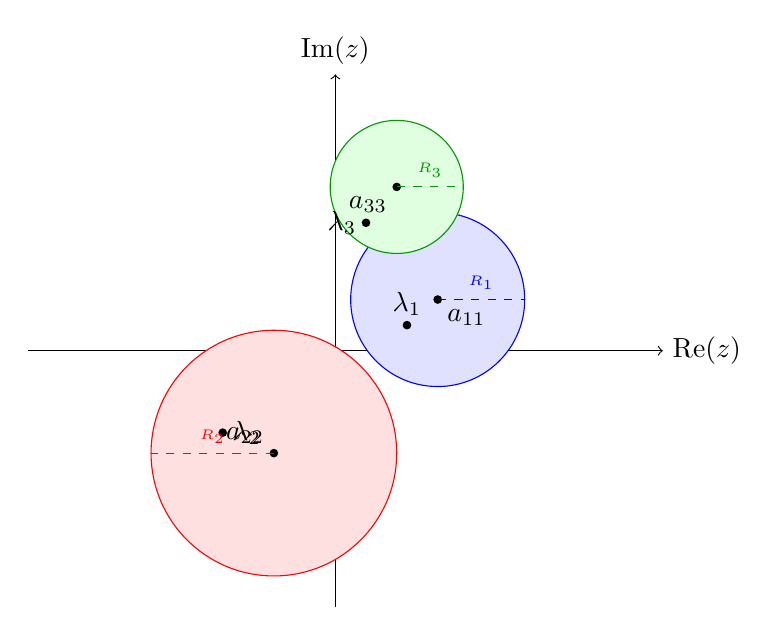
\begin{tikzpicture}[scale=1.3]
  % axes
  \draw[->] (-3.0,0) -- (3.2,0) node[right] {Re$(z)$};
  \draw[->] (0,-2.5) -- (0,2.7) node[above] {Im$(z)$};

  % centers (diagonal entries)
  \coordinate (a11) at (1.0,0.5);
  \coordinate (a22) at (-0.6,-1.0);
  \coordinate (a33) at (0.6,1.6);

  % discs
  \draw[blue, fill=blue!12] (a11) circle (0.85);
  \draw[red,  fill=red!12]  (a22) circle (1.20);
  \draw[green!60!black, fill=green!12] (a33) circle (0.65);

  % centers and labels
  \fill (a11) circle (1.2pt) node[below right] {$a_{11}$};
  \fill (a22) circle (1.2pt) node[above left] {$a_{22}$};
  \fill (a33) circle (1.2pt) node[below left] {$a_{33}$};

  % sample eigenvalues
  \fill (0.7,0.25) circle (1.2pt) node[above] {$\lambda_1$};
  \fill (-1.1,-0.8) circle (1.2pt) node[right] {$\lambda_2$};
  \fill (0.3,1.25) circle (1.2pt) node[left] {$\lambda_3$};

  % radii indicators
  \draw[blue, dashed] (a11) -- ++(0.85,0) node[midway, above, font=\tiny] {$R_1$};
  \draw[red, dashed] (a22) -- ++(-1.2,0) node[midway, above, font=\tiny] {$R_2$};
  \draw[green!60!black, dashed] (a33) -- ++(0.65,0) node[midway, above, font=\tiny] {$R_3$};
\end{tikzpicture}


    \caption{Gershgorin row discs $D(a_{ii},R_i)$ enclosing the spectrum $\sigma(A)$ in the complex plane.}
    \label{fig:gershgorin-discs}
\end{figure}

\begin{proof}[Proof sketch]
    Let $A\mathbf{v}=\lambda \mathbf{v}$, choose $m$ with $|v_m|=\|\mathbf{v}\|_\infty$. From the $m$th equation,
    \[
        (\lambda-a_{mm})v_m=\sum_{j\ne m} a_{mj} v_j, \quad \Rightarrow\quad |
        \lambda-a_{mm}|\le \sum_{j\ne m}|a_{mj}|\,\frac{|v_j|}{|v_m|}\le R_m.
    \]
\end{proof}

\begin{theorem}{Separation}{gershgorin-separation}
    If the union of discs can be partitioned into two disjoint groups $S_1, S_2$, then $A$ has as many eigenvalues (counting multiplicities) in $S_k$ as the number of discs in $S_k$.
\end{theorem}

\begin{theorem}{Boundary for irreducible matrices}{gershgorin-irreducible}
    If $A$ is irreducible and an eigenvalue lies on the boundary of one disc, then it lies on the boundary of all discs.
\end{theorem}

\begin{remark}{Homotopy and continuity}{gershgorin-homotopy}
    Consider $A(t)=D+tH$ with $D=\operatorname{diag}(a_{11},\dots,a_{nn})$ and $H=A-D$. Eigenvalues vary continuously with $t$, and Gershgorin discs track their locations from $\{a_{ii}\}$ at $t=0$ to $\sigma(A)$ at $t=1$; this provides intuition for perturbations.
\end{remark}

Convergence: subdiagonal entries $\to 0$, eigenvalues shift to diagonal.

\paragraph{Applications of the Schur Form}

\begin{itemize}
    \item Eigenvalue computation: $\lambda_i = t_{ii}$
    \item Matrix functions: $f(A) = Q f(T) Q^H$
    \item Stability analysis via triangular structure
    \item Pseudospectral computations
\end{itemize}

\begin{example}{}
    For $A = \begin{bmatrix} 1 & 2 \\ -1 & 4 \end{bmatrix}$, eigenvalues $\lambda = \frac{5 \pm \sqrt{17}}{2}$. Schur form has these on diagonal with unitary $Q$.
\end{example}

\begin{remark}{Comparison of Jordan and Schur Forms}{jordan-vs-schur}
    Jordan form reveals block structure but is numerically unstable due to sensitivity to perturbations. The
    Schur form provides stable triangularization; Jordan blocks can be inferred from $T$ but with care.
\end{remark}

\end{document}